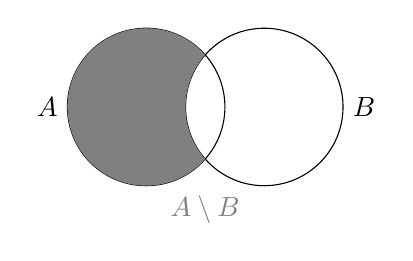
\begin{tikzpicture}
\def\firstcircle{(0,0) circle (1)}
\def\secondcircle{(1.5,0) circle (1)}

\draw \firstcircle;
\draw \secondcircle;

\node at (-1,0) [left] {$A$};
\node at (2.5,0) [right] {$B$};

\begin{scope}[even odd rule]% first circle without the second
\clip \secondcircle (-1,1) rectangle (2.5,-1);
\fill[gray] \firstcircle;
\end{scope}

\node[color=gray] at (0.75,-1) [below] {$A \setminus B$};
\end{tikzpicture}
